\section{ALGORITHM\textbackslash METHODOLOGY}
\label{sec:Algorithm}
\subsection{Path Planning Based Rolling Contact}
\noindent\uline{Rolling on discretized surfaces}:
The surface contacts between platonic solids and the plane can be categorized into three types as shown in Figure \ref{fig:gridPlatonic} including square shape for cube, triangle shape for tetrahedron, octahedron, and dodecahedron, pentagon shape for dodecahedron. 
The bottom surface of a cube occupies each square on the grid when the path planning process is executed. This property is applied for triangular grid with different rotation angle. 
In physics, the rotation angle of the cube is $\pi/2(rad)$ while the rotation angles of tetrahedron, octahedron, icosahedron and dodecahedron are $\pi-\arctan{(2\sqrt{2})}$, $\pi-2\arctan{\sqrt{2}}$, $\arccos{(-\sqrt{5}/3)}$, and $\pi-\arccos{(-\sqrt{5}/5)}$ in radian respectively.\\

\noindent{The square grid has $\pi/2$ at all corners while the triangular grid has $\pi/3$ between two arbitrary edges at a vertex. 
In the case of dodecahedron rolling contact, the Figure \ref{fig:gridPlatonic}d shows the two types of connections between pentagons where the first case has a gap (Figure \ref{fig:gridPlatonic}c) and the other has overlap pentagon connection. 
A regular pentagon has five interior angles of $\ang{108}$ which generate a gap between three pentagons surrounding because of $3*\ang{108}=\ang{324}$, which is different $\ang{360}$ of the full circle.
Another case of four overlap pentagons with $4*\ang{108}=\ang{432}$ is greater than the circle of $\ang{360}$. 
The path planning through rolling of the dodecahedron solid can be categorized into two these cases. 
It would be found the possible paths in the first case of dodecahedron without overlap rolling while the second case with overlap rolling cannot guarantee the paths.}

%
\begin{figure}[h]
\centering
	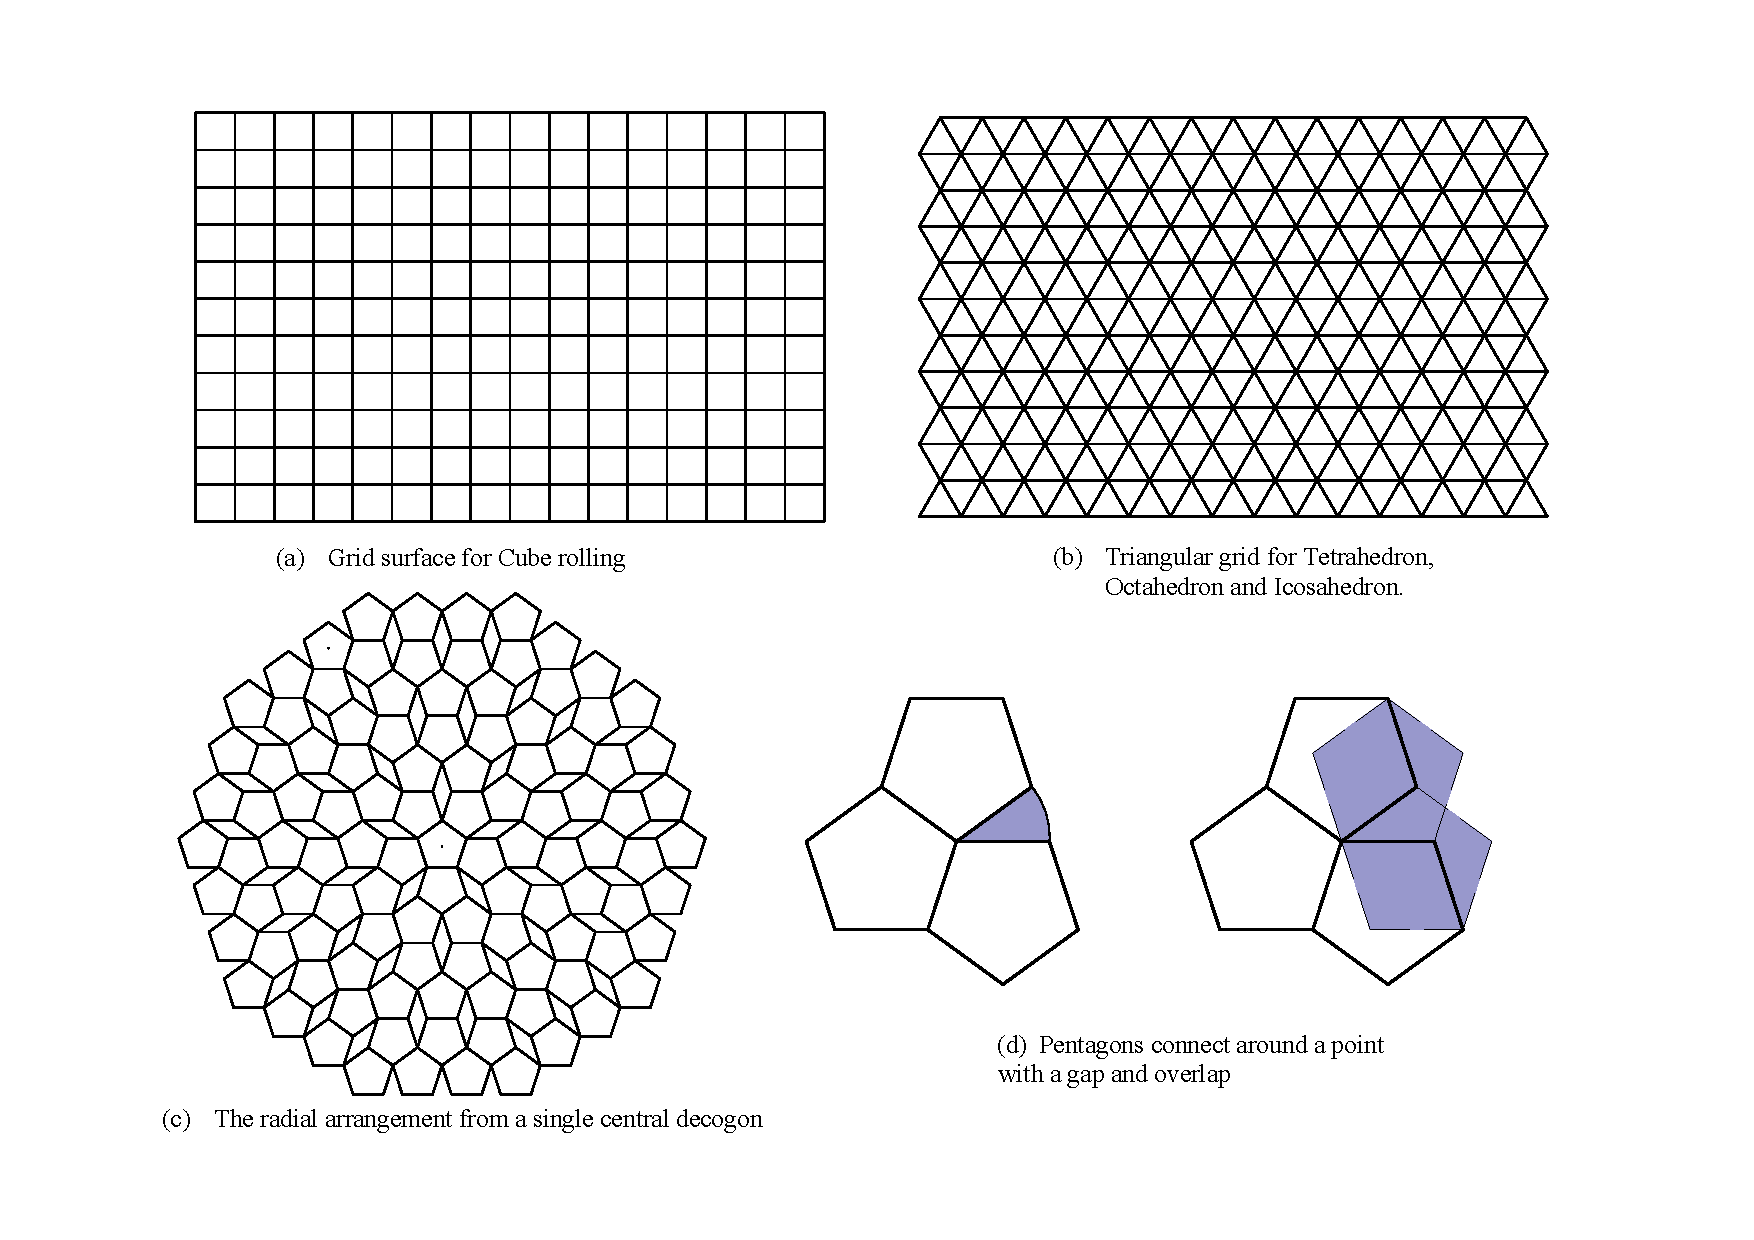
\includegraphics[width=1\textwidth]{image/gridPlatonic.pdf}
	\caption{Grid of platonic solids}
	\label{fig:gridPlatonic}
\end{figure}


\noindent\uline{Rodrigues' roatation}: It is assumed that the motion of rolling the platonic solids is a pure rolling without slipping or spinning at the line contact.
Rolling the platonic solids means rolling all its vertices in $3D$ environment indicated by changing the coordinates. There were several algorithms to transform vertices stored in a matrix in $3D$ space. In this case, the Rodrigues's rotation method in \cite{Dai_Rodrigues_2015} is used to represent the rotation matrix in the path planning algorithm. 

%The method is explained in the Section \ref{sec:eva}. \textcolor{red}{Check the paper "Kinematics of Spherical Robots Rolling Over 3D Terrains"}.

%
\clearpage
\newpage
\noindent\uline{Algorithms}:
Due to the different surface contacts, there are three types of direction for the rolling of platonic solids. As shown in the Figure \ref{fig:rollingDir}, the cube has four directions with the square surface contact while tetrahedron, octahedron and icosahedron have three rolling directions with the triangular surface contact. The dodecahedron with pentagon surface contact has five rolling directions. In the case of rolling cube, the surface contact is surrounded by four edges which means there are four possible directions through the edges. In this work, the proposed path planning algorithm deals with rolling from initial configuration within the position and orientation to the goal within the same position but different orientation. While rolling on the smooth plane, the platonic solid models will contact to the plane though their edges.\\

\noindent The Algorithm \ref{alg:rollingPath} shows that path planning for cube rolling based on tree graph search has some important steps. The first step is to initial the coordinates and the orientations of the initial cube and the target cube which is stored as the initial path. The same as tree expansion, cube will roll in four different directions including the right, left, up and down is the next step. From these new positions and orientations, the cubes will continue expand with only three directions to avoid return the previous positions. An example for this step is that from the initial coordinate the cube achieves a new position after doing rolling for right direction, the new three positions of the cube by rolling through right, up, and down direction. After implementing the expansion steps through rolling, the function of checking whether updated models reach the goal is called through the loop. By that means, the loop will stop when reaching the goal whereas the loop will continue to execute and store new models to the initial path. While the searching algorithm is executing, the data structure is used to store the positions and orientations from the start to the current. This process runs in time $O(|E|^3)$ (where $|E|$ is the number of updated cubes) which causes the longer the running time of the searching technique. \\

\noindent  
% 
%
%
%%==================================================================================
\begin{figure}[h]
\centering
	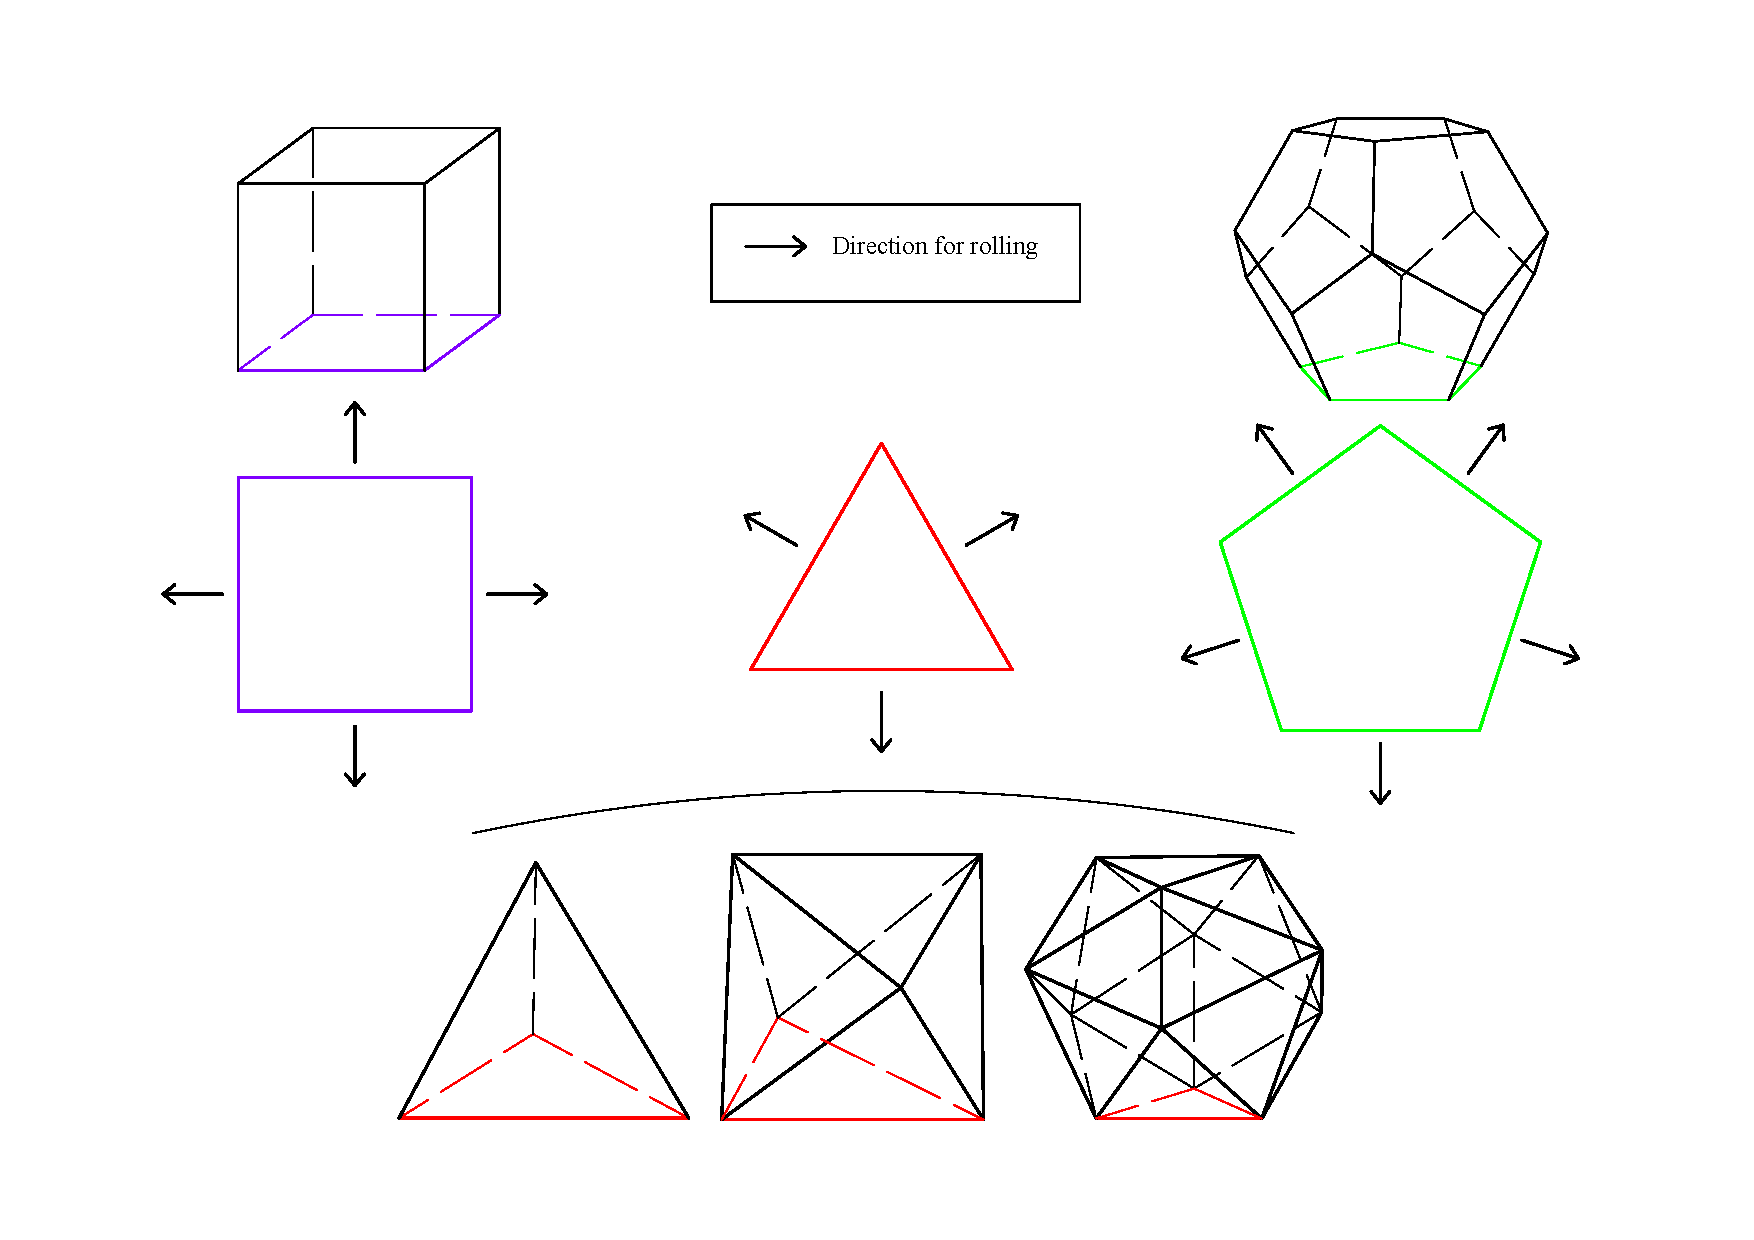
\includegraphics[width=1\textwidth]{image/rollingDir2.pdf}
	\caption{Rolling direction for each type of platonic solids}
	\label{fig:rollingDir}
\end{figure}
%
% 
%
%
%%==================================================================================
%
%
%%==================================================================================
\clearpage
\newpage
\begin{algorithm}
\caption{Path planning based rolling contact for Cube model.\label{alg:rollingPath}}
\begin{algorithmic}[1]
\Procedure {CubePathPlanning}{$S_p$, $G_p$}               \Comment{Find the shortest path from start to goal position with different orientation}
	\State $flag$ $\leftarrow$ $false$
	\State $Path[S_p]$ $\leftarrow$ $S_p$
	\State $newPoints$ $\leftarrow$ \textsc{rolling4Directions}($S_p$)	\Comment{Generate first four updated points}
	\While{$newPoints$ $!=$ $G_p$} 
		\State $updatedPoints$ $\leftarrow$ \textsc{treeExploration}($newPoints$)	\Comment{Update new three right rolling models}
		\State $n$ $\leftarrow$ \textit{size}$(updatedPoints)$
		\For{$i\gets 0, n$}		
			\For{$j\gets 1, n$}	
				\If {$updatedPoints[i]$ $=$ $updatedPoints[j]$}
					\State \textit{remove}($updatedPoints[i]$)
				\EndIf
			\EndFor
		\EndFor		
		\State $flag$ $\leftarrow$ \textsc{checkingTargetPoint}($updatedPoints$) 	\Comment{Compare updated points with goal point}  	
			\If {$flag$ $=$ $true$}
				\State \Return {$Path[S_p,G_p]$} 								    \Comment{Store new point to $Path$}
			\EndIf
			\State $newPoints$ $=$ $updatedPoints$ 
	\EndWhile
	\State  \Return {\textit{"no path found"}} 	
\EndProcedure
%\Statex
\Procedure {rolling4Directions}{$S_p$}\Comment{Generate new points in different direction of rolling}
	\State $(newRightPoint,newLeftPoint,newUpPoint,newDownPoint)$ $\leftarrow$ \textsc{rollingContact}($S_p$)				
	\State \Return{$newPoints$ $\leftarrow$ $(newRightPoint,newLeftPoint,newUpPoint,newDownPoint)$}
\EndProcedure
%%\Statex
\Procedure {treeExploration}{$newPoints$}
	\If {$dir$ $=$ $right$}
		\State  $updatedPoints$ $\leftarrow$  $(newRightPoint,newUpPoint,newDownPoint)$
	\ElsIf {$dir$ $=$ $left$}
		\State $updatedPoints$ $\leftarrow$  $(newLeftPoint,newUpPoint,newDownPoint)$
	\ElsIf {$dir$ $=$ $up$}
		\State $updatedPoints$ $\leftarrow$  $(newRightPoint,newLeftPoint,newUpPoint)$
	\Else %{$dir$ $=$ $right$}
		\State $updatedPoints$ $\leftarrow$  $(newRightPoint,newLeftPoint,newDownPoint)$
	\EndIf
	\State \Return {$updatedPoints$}
\EndProcedure
%\Statex
\Procedure {checkingTargetPoints}{$updatedPoints$,$G_p$}
	\If {$updatedPoints$ $=$ $G_p$}									\Comment{Consider both position and orientation}
		\State $flag$ $\leftarrow$ $true$
	\EndIf
	\State \Return {$flag$}
\EndProcedure
\end{algorithmic}
\end{algorithm}


%\clearpage
\newpage
%----------------------------------
\subsection{Tree Exploration Algorithm}
The node tree exploration for searching algorithm described in Algorithm \ref{alg:rollingPath} is similar to non-recursive depth-first-search algorithm. The graph search in the Figure \ref{fig:nodeTree} shows the expansion from the $root$ with node $S$ to multi-level from $1^{st} level ... n^{th} level$ for the case study of a cube solid.
%
Each node indicates the position of the cube's center and the orientation of the cube. The node $S$ means Start-Point while $R,L,U,D$ are labelled for four different directions including right, left, up and down respectively. 
%
For each iteration, a tree with a node including $3D$ coordinate and orientation is stored in each level. At the same time, the algorithm of checking the goal configuration will be called to check whether the current executing level achieves the target.\\


\noindent In other cases of tetrahedron, octahedron and icosahedron with the triangular grid (Figure \ref{fig:gridPlatonic}b), there are three directions at the first rolling and only two directions for the rest of path-finding process.
%
Only the case of dodecahedron has the different approach from the algorithm. The path planning algorithm depends on the environment including gaps or overlaps between two pentagon connections as can be seen in the Figure \ref{fig:gridPlatonic}b.
%
\vskip 0.5cm
\begin{figure}[h]
	This is the node tree for searching algorithm. Different colors indicate different level of searching steps. %\vskip 0.5cm


\tikzset{
	level/.style={sibling distance=35mm/#1},
	treenode/.style={align=center,inner sep=0pt},
	% Black nodes
	node_black/.style={treenode,circle,black,draw=black,very thick,text width=0.5cm},
	% Red nodes
	node_red/.style={treenode,circle,red,draw=red,very thick,text width=0.5cm},
	% Blue nodes
	node_blue/.style={treenode,circle,blue,draw=blue,very thick,text width=0.5cm},
	% Nil nodes
	node_nil/.style={treenode,rectangle,fill=black,minimum width=0.3cm,minimum height=0.3cm}
}
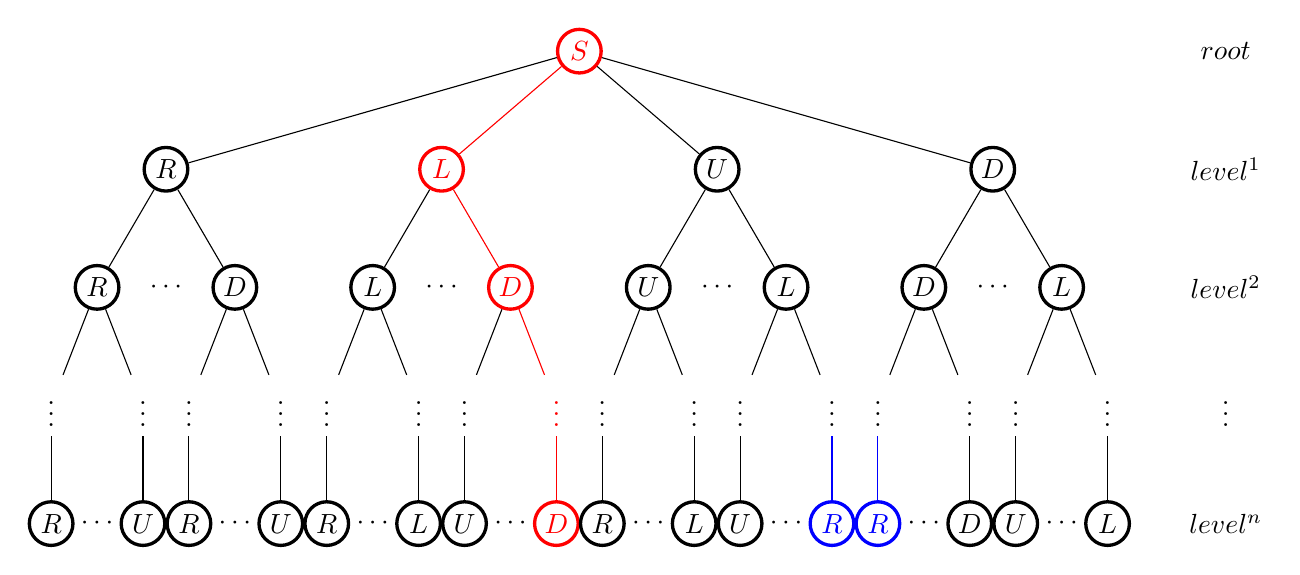
\begin{tikzpicture}
\node[node_red] (z){$S$}
  child {node[node_black] (a) {$R$}								%%% Right
    child[black] {node[node_black]  (b) {$R$}
      child {node (b1) {$\vdots$}
       child {node[node_black] (b11) {$R$}}
      }
      child {node (b2) {$\vdots$}
       child {node[node_black] (b12) {$U$}}
      }
    }
    child[black] {node[node_black] (g) {$D$}
      child {node (g1) {$\vdots$}
       child {node[node_black] (g11) {$R$}}
      }
      child {node (g2) {$\vdots$}
       child {node[node_black] (g12) {$U$}}
      }
    }
  }
   child[red] {node[node_red] (d) {$L$}                    %%%% LEft - the shortest parth
      child[black] {node[node_black]  (e) {$L$}
        child {node (e1) {$\vdots$}
         child {node[node_black] (e11) {$R$}}
        }
        child {node (e2) {$\vdots$}
         child {node[node_black] (e12) {$L$}}
        }
      }
      child[red] {node[node_red] (f) {$D$}
        child[black] {node (f1) {$\vdots$}
         child[black] {node[node_black] (f11) {$U$}}
        }
        child[red] {node (f2) {$\vdots$}
         child[red] {node[node_red] (f12) {$D$}}
        }
      }
    }
    child[black] {node[node_black] (m) {$U$}      %%% Up
      child {node[node_black]  (n) {$U$}
        child {node (n1) {$\vdots$}
         child {node[node_black] (n11) {$R$}}
        }
        child {node (n2) {$\vdots$}
         child {node[node_black] (n12) {$L$}}
        }
      }
      child {node[node_black] (o) {$L$}
        child {node (o1) {$\vdots$}
         child {node[node_black] (o11) {$U$}}
        }
        child {node (o2) {$\vdots$}
         child[blue] {node[node_blue] (o12) {$R$}}
        }
      }
    }
  child[black] {node[node_black]  (j) {$D$}   %%% Down
    child {node[node_black] (k) {$D$}
      child {node {$\vdots$}
       child[blue] {node[node_blue] (k11) {$R$}}
      }
      child {node {$\vdots$}
       child {node[node_black] (k12) {$D$}}
      }
    }
    child {node[node_black] (l) {$L$}
    child {node {$\vdots$}
     child {node[node_black] (l11) {$U$}}
    }
    child {node (c){$\vdots$}
     child {node[node_black] (l12) {$L$}
            child [grow=right] {node (r) {$level^n$} edge from parent[draw=none]
              child [grow=up] {node (s) {$\vdots$} edge from parent[draw=none]
                child [grow=up] {node (t) {$level^2$} edge from parent[draw=none]
                  child [grow=up] {node (u) {$level^1$} edge from parent[draw=none]
                   child [grow=up] {node (u) {$root$} edge from parent[draw=none]}
                                   }
                                 }
                               }
                               }
            }
          }
         }
};
\path (b) -- (g) node [midway] {$\cdots$};\path (n) -- (o) node [midway] {$\cdots$};
\path (e) -- (f) node [midway] {$\cdots$};
\path (k) -- (l) node [midway] {$\cdots$};
\path (b11) -- (b12) node [midway] {$\cdots$};
\path (g11) -- (g12) node [midway] {$\cdots$};\path (n11) -- (n12) node [midway] {$\cdots$};
\path (e11) -- (e12) node [midway] {$\cdots$};\path (o11) -- (o12) node [midway] {$\cdots$};
\path (f11) -- (f12) node [midway] {$\cdots$};
\path (k11) -- (k12) node [midway] {$\cdots$};
\path (l11) -- (l12) node [midway] {$\cdots$};
\end{tikzpicture}

%% take notes


\begin{tikzpicture}
%\node[node_black] (n12) {}
%\node[node_red] (n12) {}
%\node[node_blue] (n12) {}
\end{tikzpicture}


	\caption{Tree Exploration of Cube Rolling}
\label{fig:nodeTree}
\end{figure}

\noindent Starting form the root $S$, path planning based rolling of the cube model at the first level of expansion will generate to four different direction $R,L,U,D$. In the next level, the cube can only roll with three directions without rolling back to the previous position.  
An example of the second level is that node $R$ will roll to right, up, and down directions indicated by node $R,U,D$ respectively.\\
% 

\noindent To eliminate the processing time in the proposed algorithms, whenever any updated points achieved the same position and orientation, these nodes will merge at that $level$. An example from Figure \ref{fig:nodeTree} shows two updated nodes $R$ (blue node) at $(n-1)^{th} level$ have achieved the same position. The next path is generated from this merged nodes. 
%
From the tree exploration algorithm, the result can show only one path or various paths which depends on the initial and goal configuration. The first path is the shortest path because the executing time is shortest based on the condition of achieving goal configuration.
% 
%\vskip 0.5cm
%\begin{figure}[h]
%    \centering
%	\tikzset{
	level/.style={sibling distance=35mm/#1},
	treenode/.style={align=center,inner sep=0pt},
	% Black nodes
	node_black/.style={treenode,circle,black,draw=black,very thick,text width=0.4cm},
	% Red nodes
	node_red/.style={treenode,circle,red,draw=red,very thick,text width=0.4cm},
	% Blue nodes
	node_blue/.style={treenode,circle,blue,draw=blue,very thick,text width=0.4cm},
	% Nil nodes
	node_nil/.style={treenode,rectangle,fill=black,minimum width=0.3cm,minimum height=0.3cm}
}
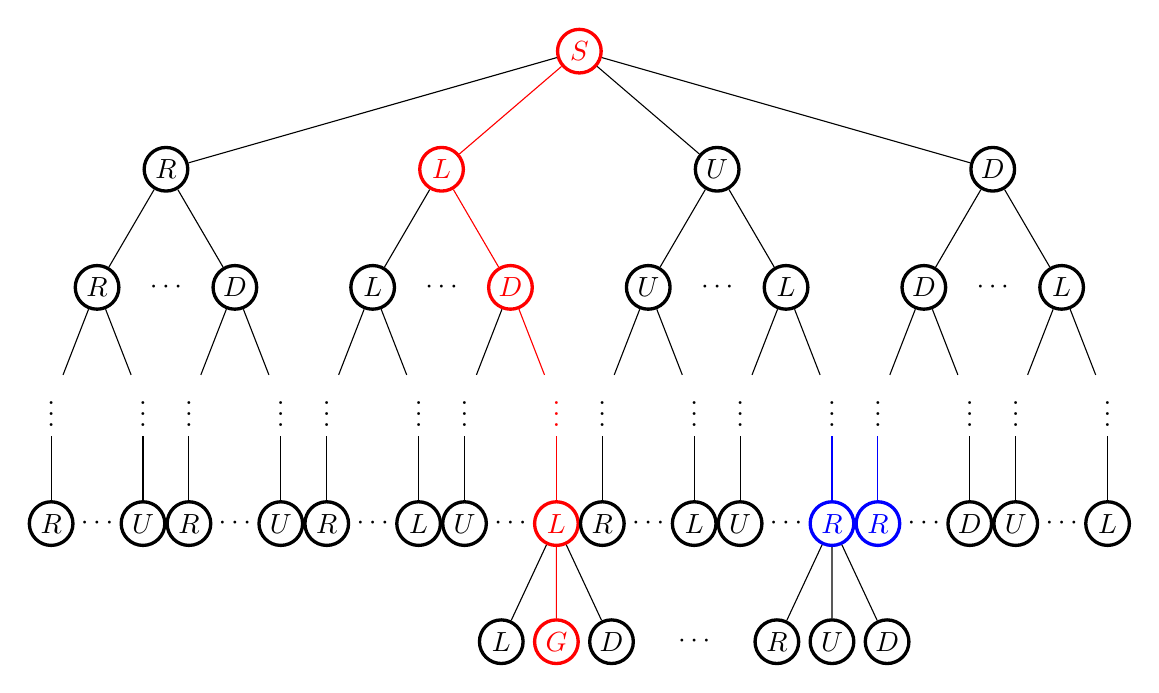
\begin{tikzpicture}

\node[node_red] (z){$S$}
  child {node[node_black] (a) {$R$}								%%% Right
    child[black] {node[node_black]  (b) {$R$}
      child {node (b1) {$\vdots$}
       child {node[node_black] (b11) {$R$}}
      }
      child {node (b2) {$\vdots$}
       child {node[node_black] (b12) {$U$}}
      }
    }
    child[black] {node[node_black] (g) {$D$}
      child {node (g1) {$\vdots$}
       child {node[node_black] (g11) {$R$}}
      }
      child {node (g2) {$\vdots$}
       child {node[node_black] (g12) {$U$}}
      }
    }
  }
   child[red] {node[node_red] (d) {$L$}         %% LEft - the shortest parth
      child[black] {node[node_black]  (e) {$L$}
        child {node (e1) {$\vdots$}
         child {node[node_black] (e11) {$R$}}
        }
        child {node (e2) {$\vdots$}
         child {node[node_black] (e12) {$L$}}
        }
      }
      child[red] {node[node_red] (f) {$D$}
        child[black] {node (f1) {$\vdots$}
         child[black] {node[node_black] (f11) {$U$}}
        }
        child[red] {node (f2) {$\vdots$}
         child[red] {node[node_red] (f12) {$L$} 
         	child[black] {node[node_black] (g44) {$L$}}
         	child[red] {node[node_red] (g22) {$G$}} 
         	child[black] {node[node_black] (g33) {$D$}}  
          }
        }
      }
    }
    child[black] {node[node_black] (m) {$U$}      %%% Up
      child {node[node_black]  (n) {$U$}
        child {node (n1) {$\vdots$}
         child {node[node_black] (n11) {$R$}}
        }
        child {node (n2) {$\vdots$}
         child {node[node_black] (n12) {$L$}}
        }
      }
      child {node[node_black] (o) {$L$}
        child {node (o1) {$\vdots$}
         child {node[node_black] (o11) {$U$}}
        }
        child {node (o2) {$\vdots$}
         	child[blue] {node[node_blue] (o12) {$R$}
         		child[black] {node[node_black] (merge1) {$R$}  }
         		child[black] {node[node_black] (merge2) {$U$}  }
         		child[black] {node[node_black] (merge3) {$D$}  }
                  }
              }
           }
    }
  child[black] {node[node_black]  (j) {$D$}   %%% Down
    child {node[node_black] (k) {$D$}
      child {node {$\vdots$}
       child[blue] {node[node_blue] (k11) {$R$}}
      }
      child {node {$\vdots$}
       child {node[node_black] (k12) {$D$}}
      }
    }
    child {node[node_black] (l) {$L$}
    child {node {$\vdots$}
     child {node[node_black] (l11) {$U$}}
    }
    child {node (c){$\vdots$}
     child {node[node_black] (l12) {$L$}
%            child [grow=right] {node (r) {$level^n$} edge from parent[draw=none]
%              child [grow=up] {node (s) {$\vdots$} edge from parent[draw=none]
%                child [grow=up] {node (t) {$level^2$} edge from parent[draw=none]
%                  child [grow=up] {node (u) {$level^1$} edge from parent[draw=none]
%                   child [grow=up] {node (u) {$root$} edge from parent[draw=none]}
%                                   }
%                                 }
%                               }
%                               }
            }
          }
         }
};
\path (b) -- (g) node [midway] {$\cdots$};
\path (n) -- (o) node [midway] {$\cdots$};
\path (e) -- (f) node [midway] {$\cdots$};
\path (k) -- (l) node [midway] {$\cdots$};
\path (b11) -- (b12) node [midway] {$\cdots$};
\path (g11) -- (g12) node [midway] {$\cdots$};
%\path (g22) -- (g33) node [midway] {$\cdots$};
\path (n11) -- (n12) node [midway] {$\cdots$};
\path (e11) -- (e12) node [midway] {$\cdots$};
\path (o11) -- (o12) node [midway] {$\cdots$};
\path (f11) -- (f12) node [midway] {$\cdots$};
\path (k11) -- (k12) node [midway] {$\cdots$};
\path (l11) -- (l12) node [midway] {$\cdots$};
\path (g33) -- (merge1) node [midway] {$\cdots$};

%\begin{tikzlegend}[legend entries={monopolist profit within entry allowance,
%      monopolist profit within entry deterrence,something else},
%        legend style={at={(0,-1)},anchor=north west}, legend cell align=left]
%     \addlegendimage{dotted,sharp plot}
%     \addlegendimage{sharp plot}
%     \addlegendimage{dashed, sharp plot}
%\end{tikzlegend}   
   
\end{tikzpicture}
%	\caption{Merge Nodes of Cube Rolling}
%\label{fig:mergeNode}
%\end{figure}
%
%----------------------------------
\clearpage
\newpage